

\begin{figure}
    \centering
    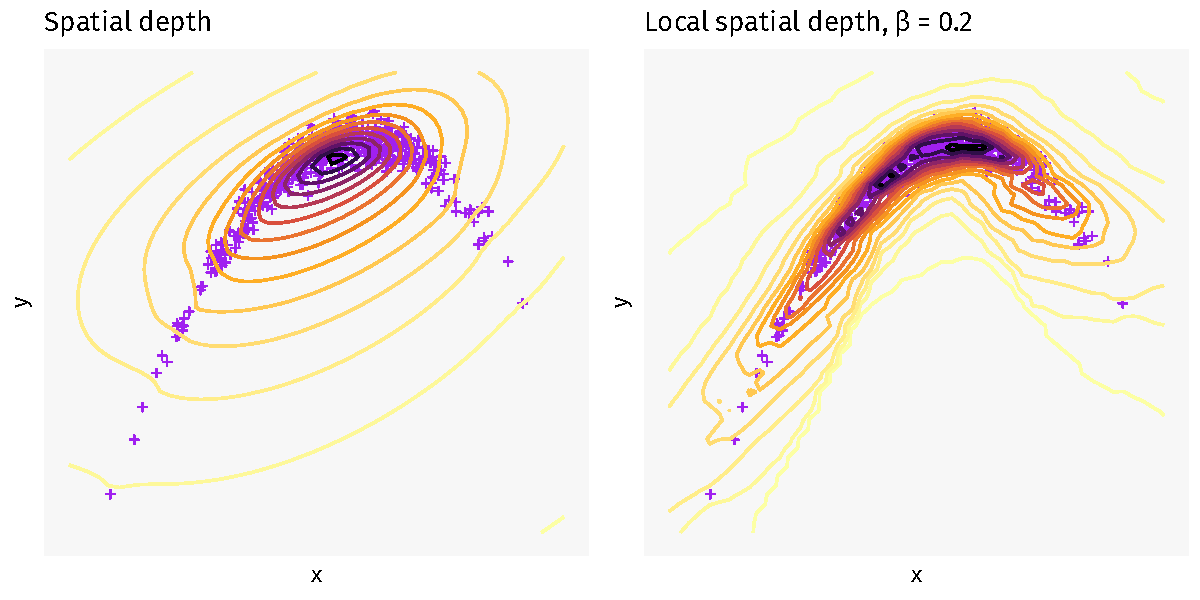
\includegraphics[width = \textwidth, page = 1]{localdepth_banana}
    \caption{
        Depth contours with respect to a `banana-shaped' distribution.
        Observe that the spatial depth contours fail to adequately capture the
        curved shape of the data cloud, in contrast with the local spatial
        depth (with $\beta = 0.2$) contours.
    }
    \label{fig:localdepth_banana}
\end{figure}



\section{Local depth regions}

Given a distribution $F_{\vX}$, we may define a symmetrized distribution about
a point $\vx \in \mathscr{X}$ as
\begin{equation}
    F^{\vx}_{\vX} = \frac{1}{2}F_{\vX} + \frac{1}{2}F_{2\vx - \vX}. \label{eq:local_symmetrization}
\end{equation}
With this, $\vx$ becomes the point of central symmetry, hence the deepest
point in $F^{\vx}_{\vX}$ with respect to a depth function $D$ that obeys
\textbf{P2}.
Thus, the $\beta$-th central regions of $F^{\vx}_{\vX}$ behave like
neighbourhoods of $\vx$.

\begin{definition}[\cite{paindaveine-bever-2013}]
    The probability-$\beta$ depth-based neighbourhood of $\vx$ with respect to
    the distribution $F$ is defined as
    \begin{equation}
        N^{\vx}_\beta(F) = C_{F^{\vx}}(\beta),
    \end{equation}
    i.e.\ the $\beta$-th central region of $F$ symmetrized about $\vx$.
\end{definition}

When working with a sample $\mathscr{D} = \{\vX_i\}_{i = 1}^n$ from $F$, we
may obtain the $\beta$ depth-based neighbourhood of $\vx$ by first computing
the reflected sample $\mathscr{D}' = \{2\vx - \vX_i\}_{i = 1}^n$, then
arranging the elements of the symmetrized sample $\mathscr{D}^{\vx} =
\mathscr{D} \cup \mathscr{D}'$ in descending order by their empirical depth
values and choosing the first $\beta$ proportion of elements.
The neighbourhood $N^{\vx}_\beta(\hat{F}_n)$ is the convex hull of these
elements.


\begin{definition}[\cite{paindaveine-bever-2013}]
    \label{def:localdepth}
    Let $D$ be a depth function, and let $F^{\vx}_\beta$ denote the
    distribution $F$ conditional on the neighbourhood $N^{\vx}_\beta(F)$.
    The corresponding local depth function at locality level $\beta \in (0,
    1]$ is defined as
    \begin{equation}
        LD_\beta(\vx, F) = D(\vx, F^{\vx}_\beta)
    \end{equation}
\end{definition}

Again, when working with a sample $\mathscr{D} = \{\vX_i\}_{i = 1}^n$, we
obtain $LD_\beta(\vx, \hat{F}_n)$ by arranging the elements of $\mathscr{D}$
in descending order by their empirical depth values in the symmetrized sample
$\mathscr{D}^{\vx}$, choosing the first $\beta$ proportion of elements, and
computing the depth of $\vx$ with respect to these elements.

\begin{remark}
    When $\beta = 1$, the local depth $LD_1$ reduces to the original global
    depth $D$.
\end{remark}

\begin{remark}
    The notions of depth based neighbourhoods and local depth make sense for
    any distribution $F$ on a space $\mathscr{X}$ as long as the process of
    symmetrization around $\vx \in \mathscr{X}$ can be achieved.
\end{remark}


\begin{figure}
    \centering
    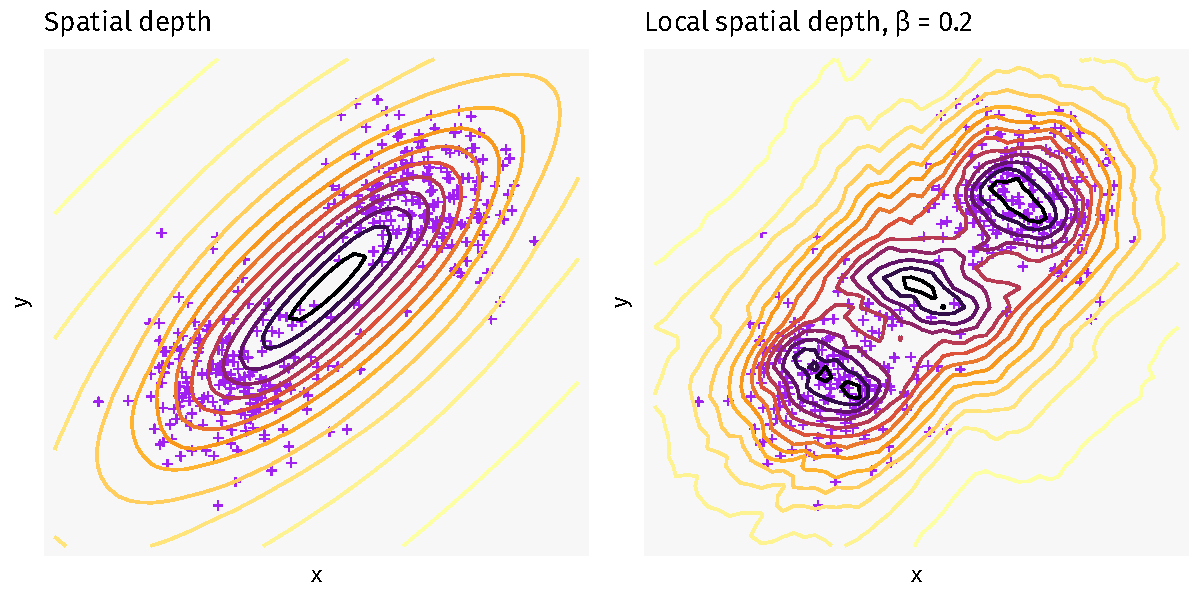
\includegraphics[width = \textwidth, page = 1]{localdepth_bimodal}
    \caption{
        Depth contours with respect to a bimodal distribution.
        Although the local spatial depth contours capture the two modes
        correctly, it erroneously ascribes high depth values to a region in
        between them.
    }
    \label{fig:localdepth_bimodal}
\end{figure}


\section{Regression based on local depth}

\begin{figure}
    \centering
    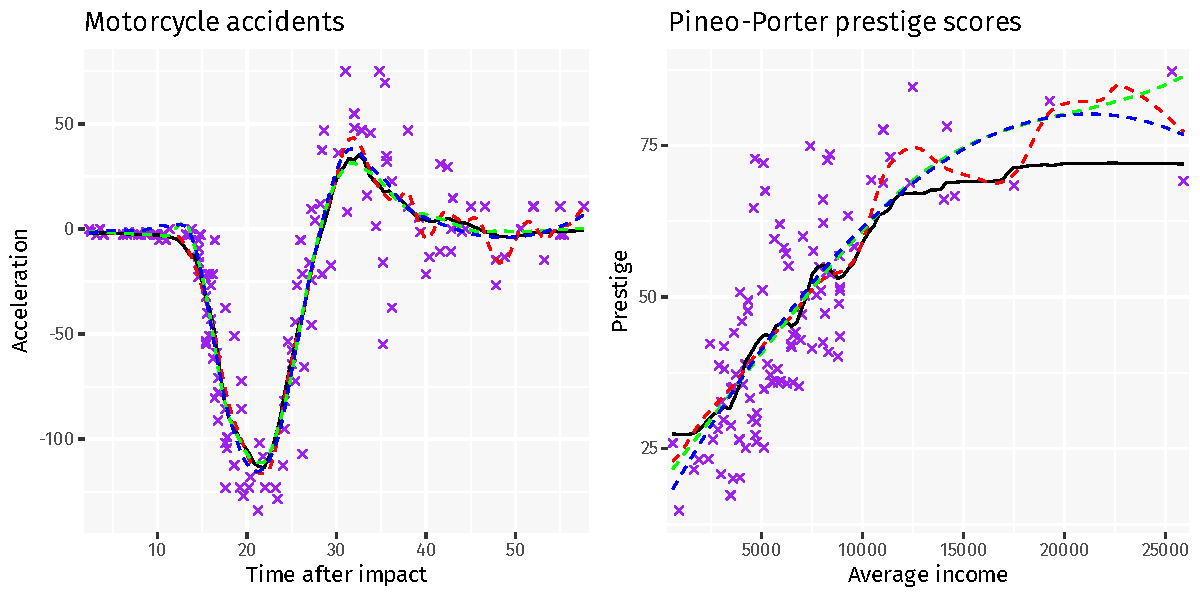
\includegraphics[width = \textwidth, page = 1]{localregression_univariate}
    \caption{
        Regression curves for the \texttt{cars} and \texttt{carData::Prestige}
        datasets available in R.
        The black curve indicates the local depth based estimate, the dashed
        red curve indicates the Nadaraya-Watson kernel based estimate, and the
        dashed green and blue curves indicate the local linear and quadratic
        estimates respectively.
        The locality levels and relevant bandwidths have been obtained by
        leave-one-out cross validation.
    }
    \label{fig:localregression_univariate}
\end{figure}

\begin{definition}
    Let $D$ be a depth function, and let $\tilde{F}^{\vx}_\beta$ denote the
    symmetrized distribution $F^{\vx}$ conditional on the neighbourhood
    $N^{\vx}_\beta(F)$.
    Given $\vx \in \mathscr{X}$, we may define a local depth kernel at
    locality level $\beta$ centered at $\vx$ as
    \begin{equation}
        K^{\vx}_\beta\colon N^{\vx}_\beta(F) \to \R, \qquad
        \vz \mapsto D(\vz, \tilde{F}^{\vx}_\beta).
    \end{equation}
    This naturally extends to a map $\mathscr{X} \to \R$ as
    $K^{\vx}_\beta(\vz) = 0$ for $\vz \notin N^{\vx}_\beta(F)$.
\end{definition}

Note that $\tilde{F}^{\vx}_\beta$ is angularly symmetric about $\vx$.
As a result, $K^{\vx}_\beta$ is maximized at and decreases away from $\vx$,
for reasonably well behaved depth functions (\textbf{P2} and \textbf{P3} for
multivariate depth functions).


With this, we propose the (linear) estimator
\begin{equation}
    \hat{\vy}_\beta(\vx) = \sum_i w_i(\vx)\, \vy_i, \qquad
    w_i(\vx) = \frac{K^{\vx}_\beta(\vx_i)}{\sum_j K^{\vx}_\beta(\vx_j)}.
    \label{eq:localregression}
\end{equation}
The locality level $\beta \in (0, 1]$ is a tuning parameter which may be
chosen via methods such as cross-validation.

The kernel function $K^{\vx}_\beta$ is supported on the neighbourhood
$N^{\vx}_\beta(F)$, whose shape may vary with changing $\vx \in \mathscr{X}$.
Indeed, since $N^{\vx}_\beta(\hat{F}_n)$ contains the $\beta$ proportion of
points from $\{\vx_i\}$ `closest' to $\vx$ (in the sense of being more central
in the symmetrized dataset $\mathscr{D}^{\vx}$), this neighbourhood ought to
be smaller when $\vx$ is more central, and larger when $\vx$ has fewer points
nearby.
Thus, $K^{\vx}_\beta$ behaves somewhat like a variable bandwidth kernel, whose
shape adjusts to the dataset.
Furthermore, the `bandwidth' of $K^{\vx}_\beta$ is controlled solely by the
parameter $\beta$ regardless of the dimensionality or nature of $\mathscr{X}$.
This stands in contrast with more traditional kernels which often require a
selection of multiple bandwidths.
For instance, a Gaussian kernel of the form
\begin{equation}
    \vz \mapsto \exp\left(-\sum_i \frac{(x_i - z_i)^2}{2h_i^2}\right)
    \label{eq:kernel_gaussian}
\end{equation}
needs $d$ parameters $\{h_i\}_{i = 1}^d$ to be determined.

Equation~\ref{eq:localregression} may also be thought of as a weighted KNN
estimator, since $N^{\vx}_\beta(\hat{F}_n)$ always captures the same number of
points.

When the depth function $D$ is chosen to be affine invariant, the estimator
\ref{eq:localregression} is also affine invariant, in the sense that it is
unchanged by an affine transformation of $\mathscr{X}$.
This is because $N^{A\vx + \bm{b}}_\beta(F_{A\vX + \bm{b}})$ will simply be
the affine image of $N^{\vx}_\beta(F_{\vX})$.
